\documentclass{article}
\usepackage[utf8]{inputenc}
\usepackage{natbib}
\usepackage{graphicx}
\usepackage{amsmath}
\usepackage{amssymb}

\begin{document}
\vspace*{-1cm}

\includegraphics[width=2cm]{logo}
\vspace*{-2cm}

\hspace*{2cm}
 \begin{tabular}{l}
	{\sc Pontificia Universidad Católica de Chile}\\
  {\sc Escuela de Ingeniería}\\
  {\sc Departamento de Ciencia de la Computación}\\
  {\sc }
 \end{tabular}
\hfill
\vspace*{-0.2cm}
\hspace*{2cm}
\begin{center}{IIC2115-Programación Como Herramienta para la Ingeniería} \\
\vspace*{3mm}
{\Large\bf Laboratorio 4}\\
\vspace*{3mm}
{Iván Santibañez\\
{Pilar Prieto}\\
\vspace*{1mm}
\end{center}
\hrule\vspace*{2pt}\hrule
\section*{Diagrama del modelo de la base de datos}
Para realizar el laboratorio se crearon 4 tablas distintas a partir de la base de datos, junto a 3 tablas relacionales que unen las llaves (elementos únicos) de aquellas que tienen alguna relación entre si. 
Las tablas creadas fueron las siguientes:
\begin{itemize}
    \item Aplicaciones: Contiene un id único por aplicación junto el rating, reviews, tamaño, instalaciones, tipo, precio, última actualización, versión actual y version android. 
    \item Géneros: Contiene un id único por género y el nombre del género. 
    \item Categorías: Contiene un id único por categoría y el nombre de la categoría. 
    \item Reviews: Contiene un id único por reseña, el texto de la reseña, sentimiento asociado, la polaridad y subjetividad del sentimiento.
\end{itemize}
En la figura 1 se presenta el diagrama del modelo explicado, donde cada tabla es presentada con un color distinto, y los rombos representan las tablas relacionales que unen los elementos únicos de cada tabla. 
\begin{figure}[h]
\centering
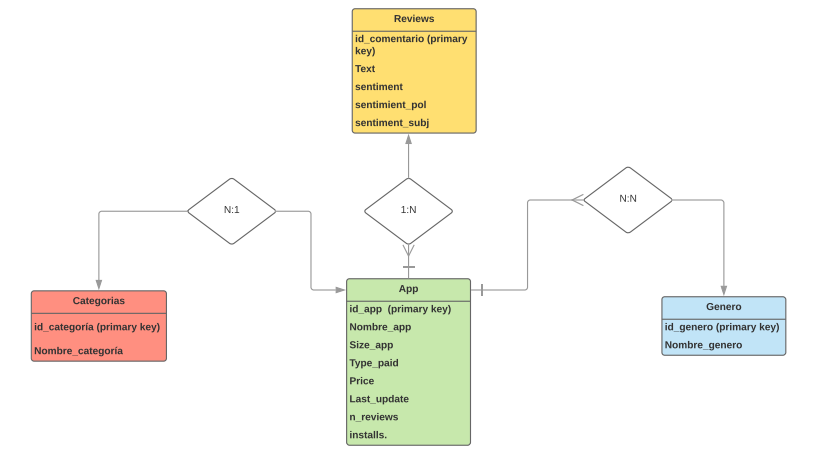
\includegraphics[width=1.2\textwidth]{Modelo.PNG}
\caption{\footnotesize{Diagrama base de datos.}}
\end{figure}
\section*{Justificación}
Las tablas fueron elegidas de tal forma de que los datos no se repitieran entre ellas, es decir, que si una aplicación tiene N comentarios, que no se repita en una misma tabla N veces el nombre de la aplicación. A a la vez, se buscó que fueran de ayuda para realizar las consultas más facilmente.\\
Dado que cada una de las aplicaciones tiene características propias de ellas y que varían mucho entre las distintas aplicaciones, se dejaron estos items en la tabla (como el precio, el tamaño, numero de instalaciones). No tenía mucho sentido crear nuevas tablas con los datos ya que no aportaba al acceso a la información.\\
Por otro lado, dado que los géneros y las categorías se repiten mucho entre las aplicaciones, y a que muchas de las consultas hacían referencia a ellos, se crearon estas dos tablas aparte con los nombres de cada categoría y de cada género. Las consultas "best by genre", "price of the best by genre", y "recommend" utilizan la tabla de géneros, lo que hace la busqueda más ordenada y directa. Por otro lado, la consulta "need update" utiliza la tabla de categorías.\\
En cuanto a la tabla de reviews, se hace necesario tener una tabla aparte, ya que son muchos los comentarios por aplicación, por lo que unirlo a la tabla de aplicaciones haría que los datos se repitan muchas veces. Al hacer un id de cada comentario y relacionarlo con el id de la aplicación que corresponde, hace que el uso de las tablas sea nuevamente más simple y ordenado.\\
Por lo tanto, podemos afirmar que el modelo elegido es adecuado ya que cada una de las tablas contiene datos únicos (id no se repiten), que se relacionan entre si mediante tablas auxiliares, y por último la forma en la que se definieron las tablas hace que la implementación de las consultas sea más simple. 



\end{document}